\chapter{多用途边界处理}
\label{sec:siga21}

% Sec 3.1
\section{动机}
流固耦合对于复杂的视觉现象仿真有很重要的作用,流体和固体之间的相互作用对两者的运动皆有影响,从而成为一个时间上的迭代过程。这种相互作用在数值上的计算是非常复杂的,并且,在有薄壳或细棒的场景中,流固耦合的计算是更加艰巨的。我们这里定义的薄壳或细棒是在某一个或某两个维度上非常狭窄的物体,以至于在这些维度上,物体的大小是远小于网格的尺度的。由于薄壳或细棒的这种特性,它们的特征在网格中很难被捕捉到,以至于经常发生泄漏或穿透等现象。

虽然有工作展示了薄壳~\cite{DiscreteShells,Bridson:2003} 或细棒~\cite{DiscreteRods} 的仿真,也包括它们在黏性流体~\cite{Fei-2018,Takahashi:2019,Fei-2019} 或非湍流~\cite{Azevedo-2016} 中的耦合,在动力学方法中使用扩散界面浸入边界法可以在湍流中或者更加稳定、高效的仿真结果~\cite{Li-2018,Li-2020}。

在本章中,我们介绍一个在LBM框架下的高效且通用的双向流固耦合边界处理方法,以可同时求解固体任意维度为亚网格尺度的情况。我们的方法将简单反弹边界方法与一个速度修正方法混合,以克服之前方法的缺点,提升仿真的稳定性与视觉效果。并且,通过几何上的近似,与实现层面的GPU优化,我们的方法相比Chen等~(\citeyear{Chen-2021}) 提出的LBM优化方案,在仿真效率上有着数倍的提升。

因为LBM使用笛卡尔网格来离散空间空间,而固体的边界一般不与网格对齐,于是出现了切削网格的概念,即网格被固体边界所切割,如图~\ref{img:cutcell_and_interpolation} 中的绿色网格。一般在LBM中需要对切削网格进行特殊处理,以刻画流体与固体间的相互作用。现有的各类基于切削网格的边界处理方法虽不能在效率、准确度、稳定性上都尽善尽美,但也有各自的优势。如扩散界面浸入边界法不需要追踪网格随物体的变化,从而降低了求解的复杂度。但它通过施加惩罚力来描述边界对流体的作用,不能准确刻画边界的形状,从而不适用于薄物体的仿真,如图~\ref{img:cutcell_and_interpolation} 所示。而简单反弹边界方法虽然可以通过分布函数的反弹阻止流体泄露 (即使是薄物体),但是因为它的准确性有限,在仿真中会产生不正确的速度分布,影响仿真的稳定性,如图~\ref{img:Immersed_Bounce_back}所示。

我们提出混合方法的一个重要动机是,这两类方法实质上是互补的。在反弹边界方法中,介观尺度的分布函数反弹从宏观上看,构成了部分浸没边界法中所需的惩罚力。而其本身又有着可以防止流体穿过薄物体的性质,所以我们可以施加一个额外的辅助惩罚力,对反弹边界法进行修正。我们注意到这个辅助惩罚力会比浸没边界法中原本的惩罚力要小很多。这样的混合方法可以满足我们在正确求解薄物体的同时,对精度与效率的需要。

\begin{figure}[htb]
    \centering
      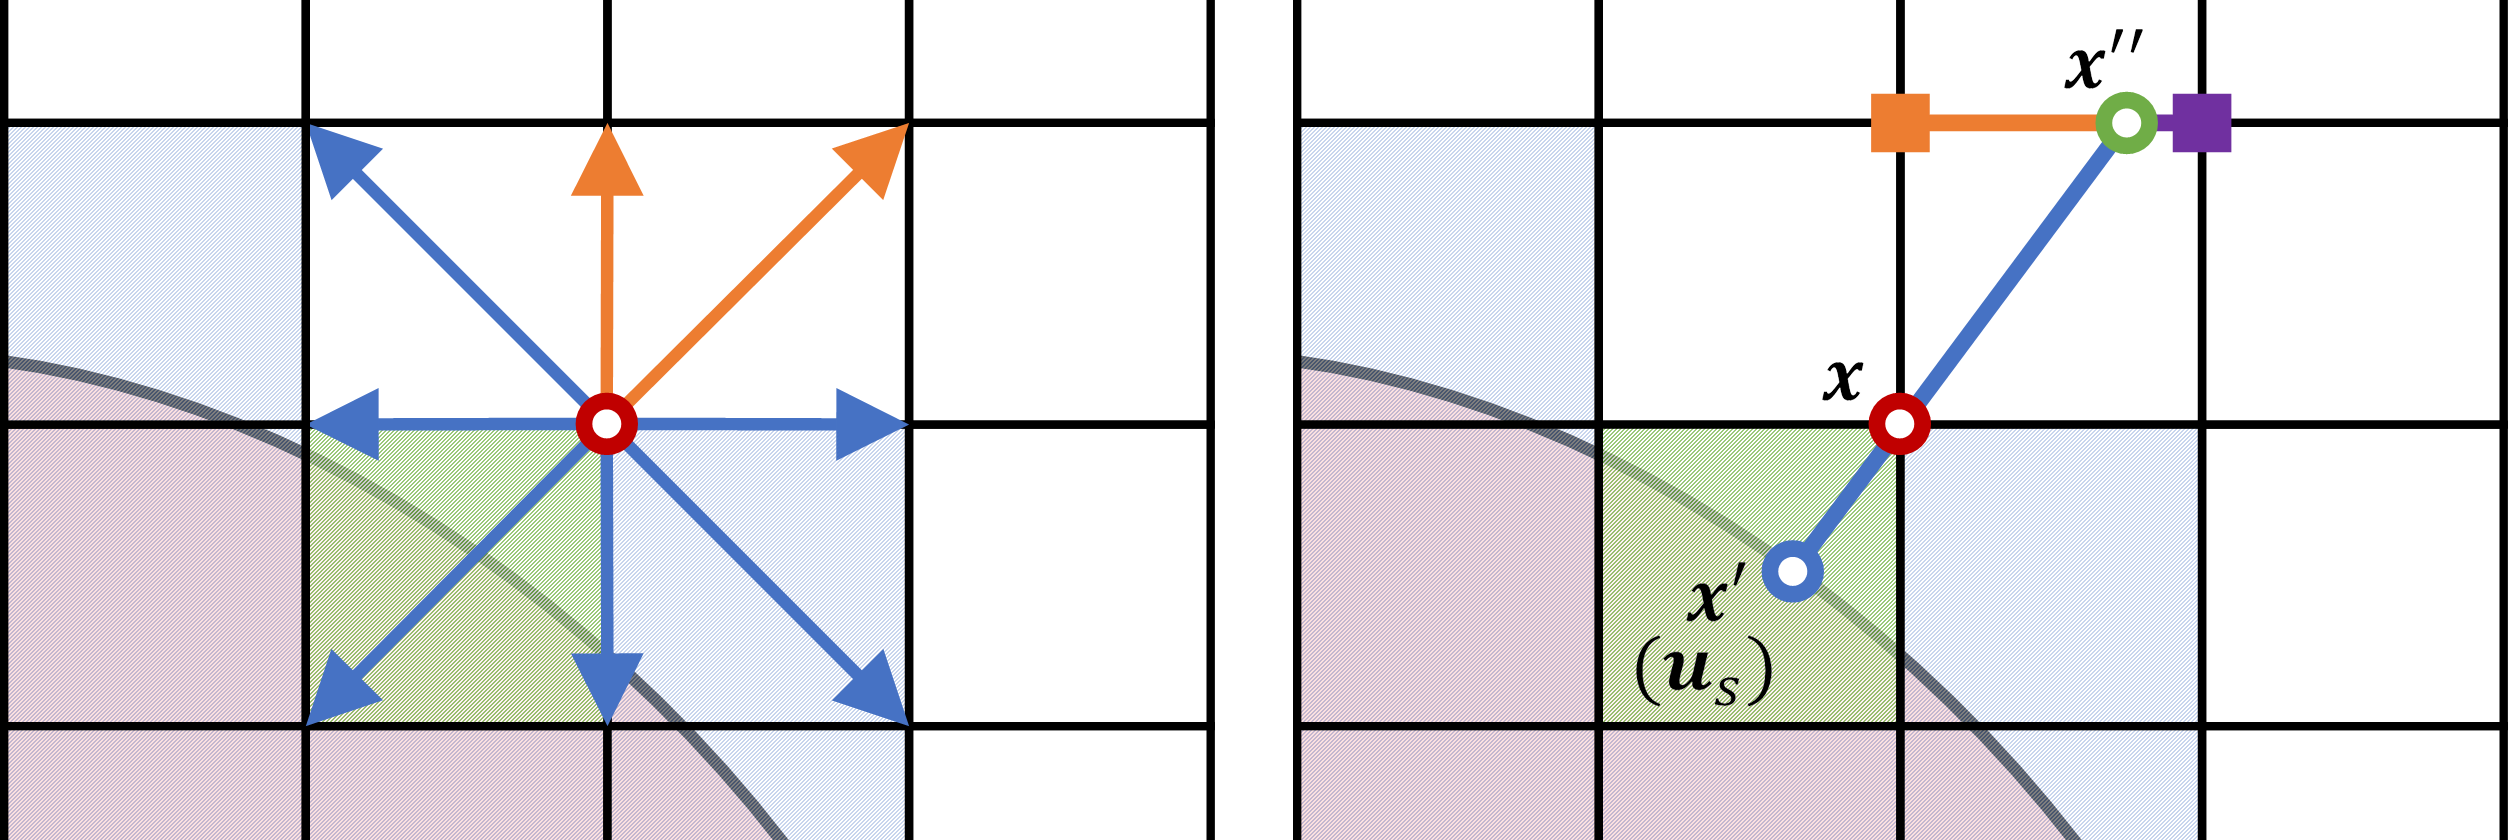
\includegraphics[width=0.95\columnwidth]{figures/cutcell_and_interpolation.png}
    \bicaption{切削网格中的速度插值。左图:因为固体边界存在而产生的切削网格 (图中标为绿色)。右图:流体中的切削网格格点$\bm{x}$ (图中标为红色圆圈) 的速度,需要通过固体边界的投影点$\bm{x}{'}$ (图中标为蓝色圆圈),与该投影点到格点的延长线与下一个网格的交点$\bm{x}{''}$ (图中标为绿色圆圈) 进行速度的线性插值得到。}{Interpolation of velocity on cut-cell nodes. Left: cut-cell (marked in green) intersecting a solid boundary; Right: the velocity on a cut-cell node $\bm{x}$ inside the fluid region (red circle) needs to be interpolated using the velocities of its projected point $\bm{x}{'}$ onto the solid boundary (blue circle) and the intersected point between the ray from the projected point to the cut-cell node and the interpolated fluid point $\bm{x}{''}$ (green circle), where the velocity can be reliably evaluated through simple linear interpolation.}
    \label{img:cutcell_and_interpolation}
\end{figure}

\begin{figure}[htb]
    \centering
      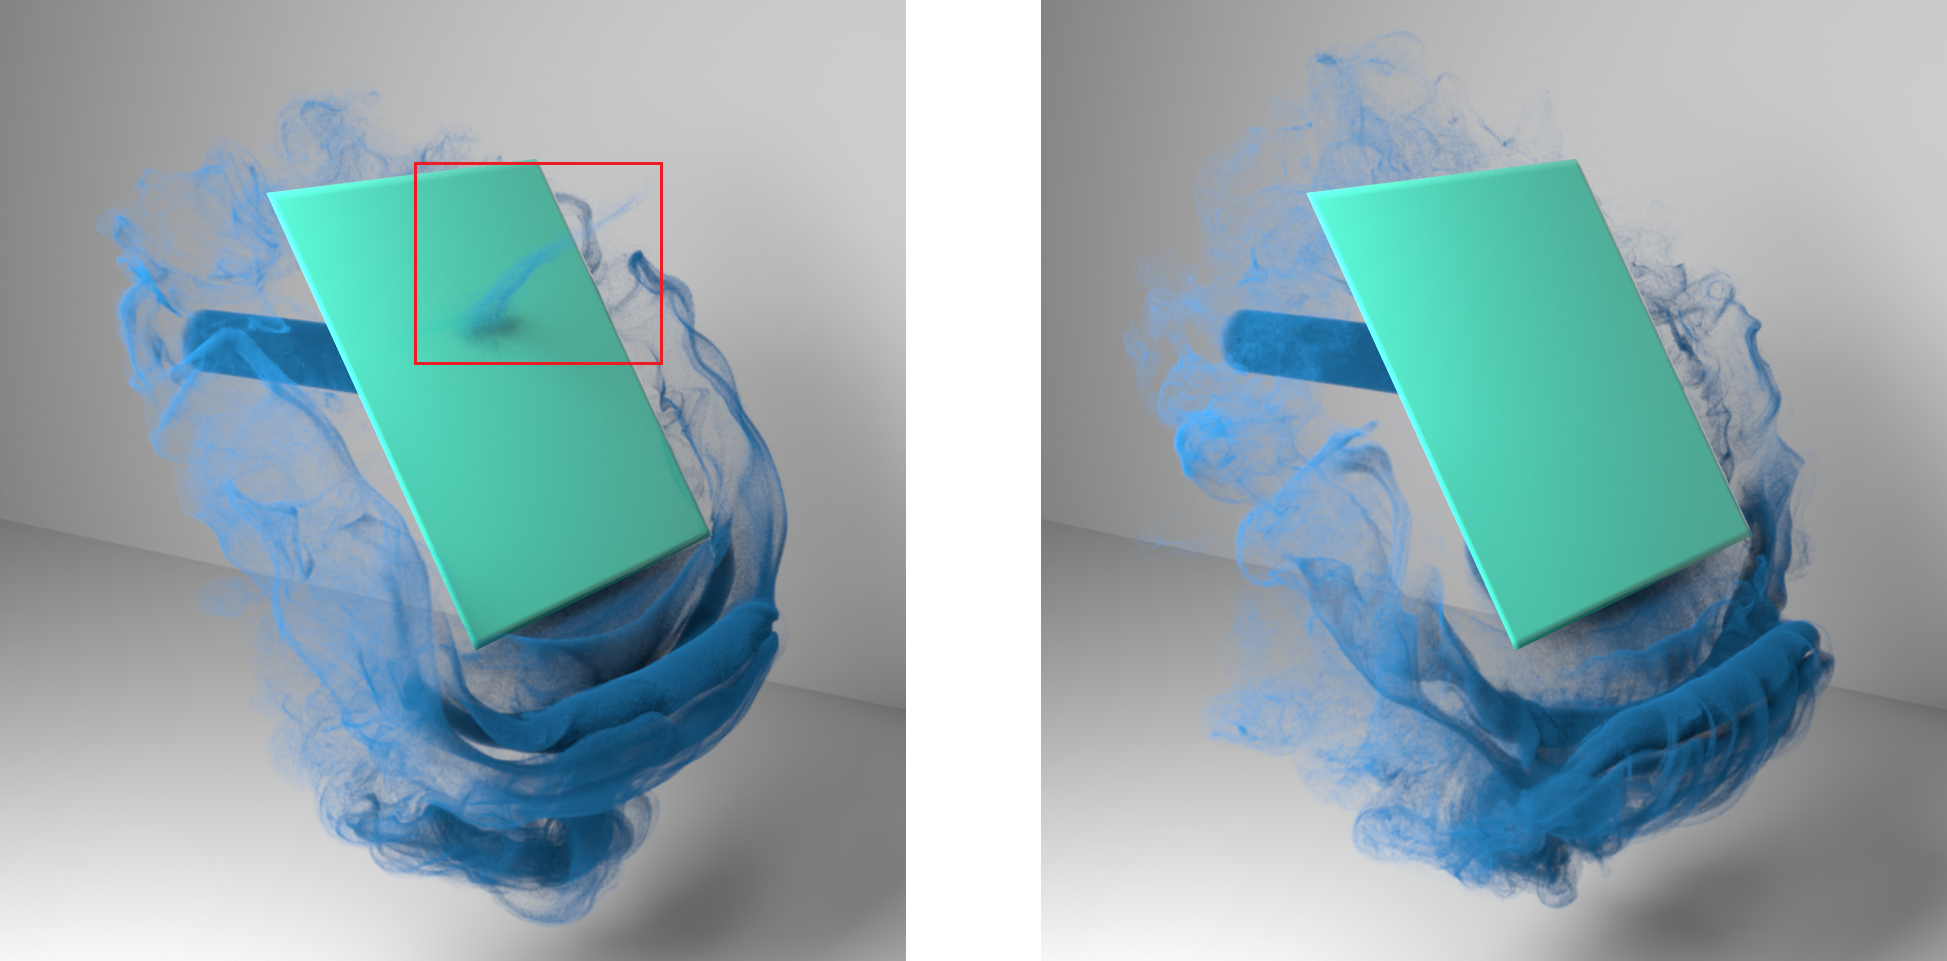
\includegraphics[width=0.97\columnwidth]{figures/comparison_with_ib.png}
    \bicaption{浸没边界法造成的泄露。当有薄板存在时,Li等~(\citeyear{Li-2020}) 所使用的浸没边界法 (左图) 与我们的方法的对比 (右图)。因为惩罚力会分布到薄板两侧,扩散边界浸没边界法可能会产生泄露 (见图中红色方框),而我们的方法可防止此现象。}{Leakage of immersed boundary. For a kinetic fluid simulation coupled with a thin plate, the immersed boundary method used by Li et al.~(\citeyear{Li-2020}) (left) is compared with our method (right). Due to force spreading in both sides of the thin plate, this recent coupling approach employing a diffuse-interface immersed boundary method may generate leakage through the plate (see red box), while our method prevents this issue by design.}
    \label{img:comparison_with_ib}
\end{figure}

\begin{figure}[htb]
    \centering
      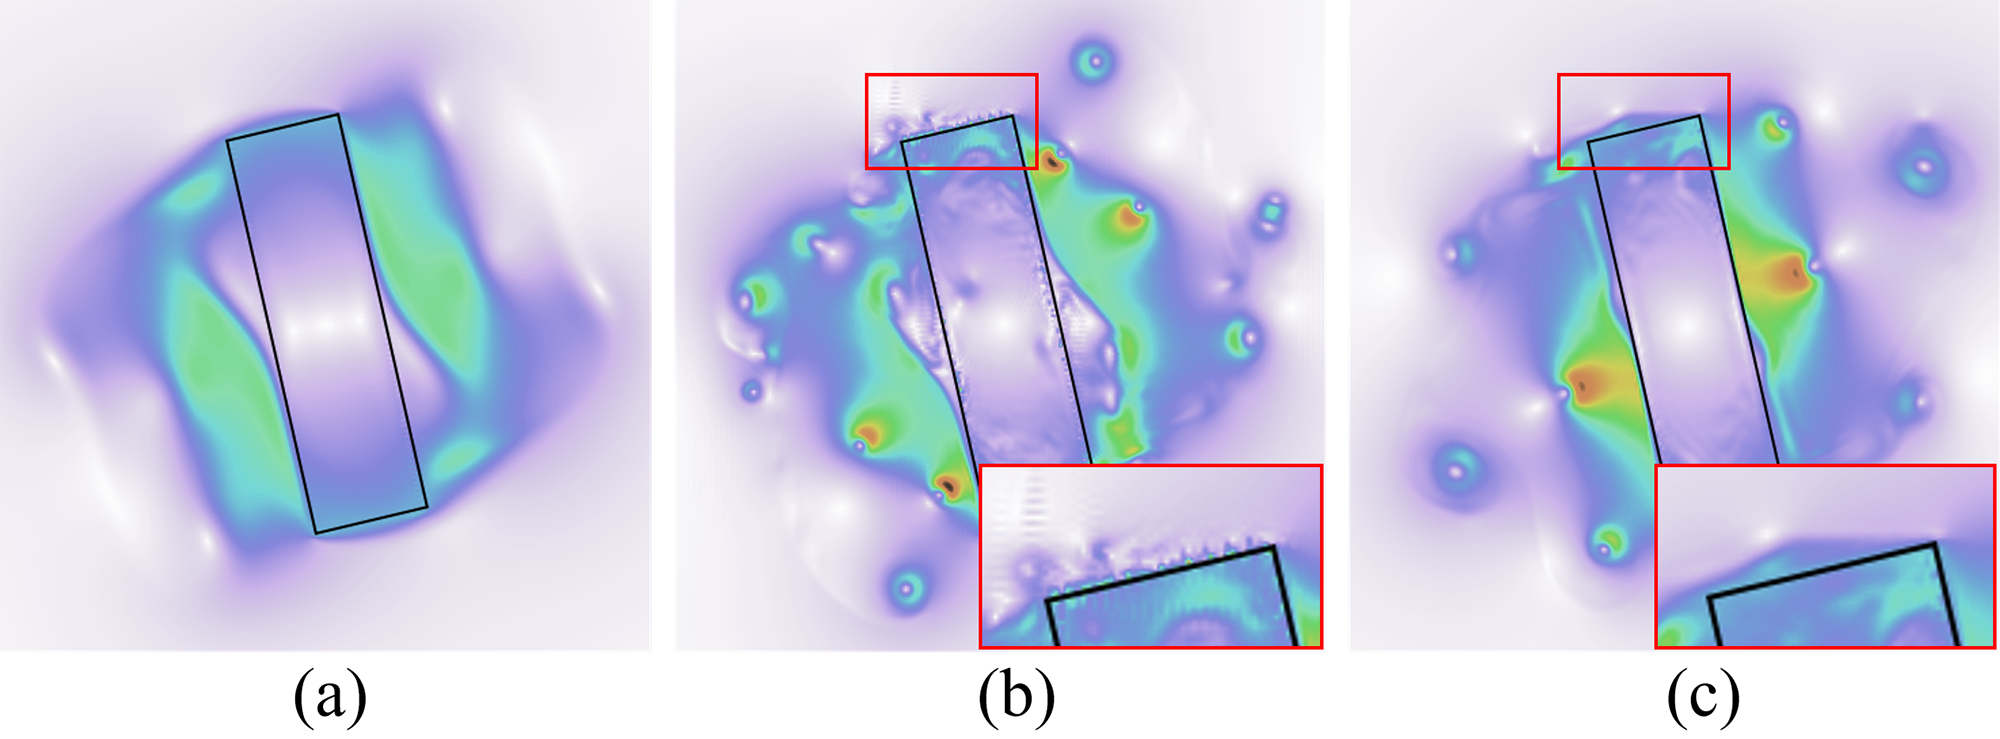
\includegraphics[width=0.95\columnwidth]{figures/ib-mbb.png}
    \bicaption{不同雷诺数下的简单反弹边界处理方法。(a) 在低雷诺数下,简单反弹边界没有造成视觉不正确的现象;(b) 但在高雷诺数下,固体边界会有很强的锯齿现象,从而对稳定性有较大影响;(c) 我们的方法在与 (b) 同样的高雷诺数情况下看不到视觉不正确的现象。}{Simple bounce-back under different Reynolds numbers. (a) a plain simple bounce-back scheme generates no visual artifacts for  flows with low Reynolds number; (b) however, it exhibits strong aliasing artifacts near the solid boundary for high Reynolds number flows, which may seriously influence stability; (c) our new boundary treatment for the same high Reynolds number as in (b) is artifact-free, generating the type of vortices expected from such an example.}
    \label{img:Immersed_Bounce_back}
\end{figure}

% Sec 3.2
\section{方法}
我们的混合方法主要包含下面三个部分:
\begin{itemize}
\item 双面简单反弹边界:我们首先介绍一个简单反弹边界方法的变种,即切削网格边界的两侧都会发生分布函数的反弹,而不只在一侧发生,从而不再需要追踪格子随物体运动的状态变化;
\item 切削网格的速度修正:我们通过在切削网格内进行单边的速度修正,大幅提升仿真的稳定性,同时压制边界上的速度误差;
\item 固体受力:最后我们通过介观与宏观的混合,求出流体转移至固体的动量,从而获得固体受力以驱动固体运动。
\end{itemize}

我们将在下面依次介绍这三部分内容。

\subsection{双面简单反弹边界}
在第~\ref{sec:boundary_treatment} 节中,我们回顾了简单反弹边界方法。一般来说,反弹边界都只应用于流体点。然而随着物体的运动,流体点可能被固体覆盖成为固体点,固体点也可能重新变为流体点。这个转换过程不止需要追踪格点状态,并且需要进行速度的插值,甚至外插。这样会在高雷诺数下在固体边界上产生很强的耗散误差。为了避免这一现象,我们对所有切削网格内的点都进行分布函数反弹,而不只针对流体点。我们称该方法为\emph{双面简单反弹边界方法}。该方法依旧可以避免流体泄露,即使有亚网格物体存在。但这并没有改善固体边界的速度锯齿现象与大速度梯度造成的误差,所以我们引入下一节中介绍的速度修正方法。

\subsection{切削网格的速度修正}
因为我们谋求的是低阶 (线性) 精度的边界处理,我们提出在双面简单反弹边界之后,通过沿固体边界的法向方向对速度线性插值,来对速度场进行修正。修正的方式为对流场施加惩罚力。更具体地说,我们先通过切削网格点周围的固体和流体速度插值,得到一个切削网格点上的期望速度。之后通过当前速度与期望速度的差计算惩罚力,从而修正速度场。

\paragraph{切削网格点上的期望速度}
切削网格点上的期望速度可通过其邻近的可靠速度插值得来。对于处于固体内部的切削网格点,它们的期望速度必须与那一点的固体速度一致,这个速度可以通过固体的运动状态直接获得。
对于流体中的切削网格点,我们通过一个线性插值,获得其期望速度。该插值方法如图~\ref{img:cutcell_and_interpolation} 中右图所示。对于切削网格点$\bm{x}$点,我们首先计算它在固体边界的投影点位置$\bm{x}'$,之后从$\bm{x}'$向$\bm{x}$打一条射线,该射线与下一个网格面的交点为$\bm{x}''$。如果这个面上的所有点都不是切削网格点,$\bm{x}''$点的速度就可以通过该面上的点线性插值得来 (二维中是线性插值,三维中是双线性插值)。如果这个面上存在点是切削网格点,则可寻找下一个交点,直到找到满足条件的交点。此时$\bm{x}$点的期望速度则可通过线性插值得到:
\begin{equation}  \label{eq:vel_lerp}
\hat{\bm{u}}(\bm{x})=(1-\alpha)\bm{u}_s + \alpha \bm{u}(\bm{x}'')\;,
\end{equation}
其中$\alpha=\|\bm{x}-\bm{x}'\|/\|\bm{x}''-\bm{x}'\|$,$\bm{u}_s$是固体边界上投影点$\bm{x}'$的速度。

\paragraph{基于惩罚力的速度修正}
% From an expected velocity $\hat{\bm{u}}(\bm{x})$ at a cut-cell node $\bm{x}$, which may differ from its current post-bounce velocity $\bm{u}(\bm{x})$, we derive a penalty force $\bm{F}_p(\bm{x})$ as\vspace*{-1mm}
% \begin{equation} \label{eq:penaltyForce}
% \bm{F}_p(\bm{x}) = \hat{\bm{u}}(\bm{x})-\bm{u}(\bm{x})\;,\vspace*{-1mm}
% \end{equation}
% which we apply as an external force to node $\bm{x}$. As done in the LBM solver of~\cite{Li-2020}, we first project the penalty force onto the space of discrete distribution functions using the highest-order Hermite polynomial expansion in order to retain accuracy and stability. Note that compared to the traditional IB methods, these ancillary penalty forces are far weaker: our double-sided bounce-back scheme applied earlier already accounted for a large part of the boundary condition enforcement, so the forces are just a further adjustment of the velocity.
% Thus, one does not need to reduce the physical time step via time rescaling, and a faster coupling simulation is achieved than with the traditional IB approach used in~\cite{Li-2020}.

\begin{figure}[htb]
    \centering
      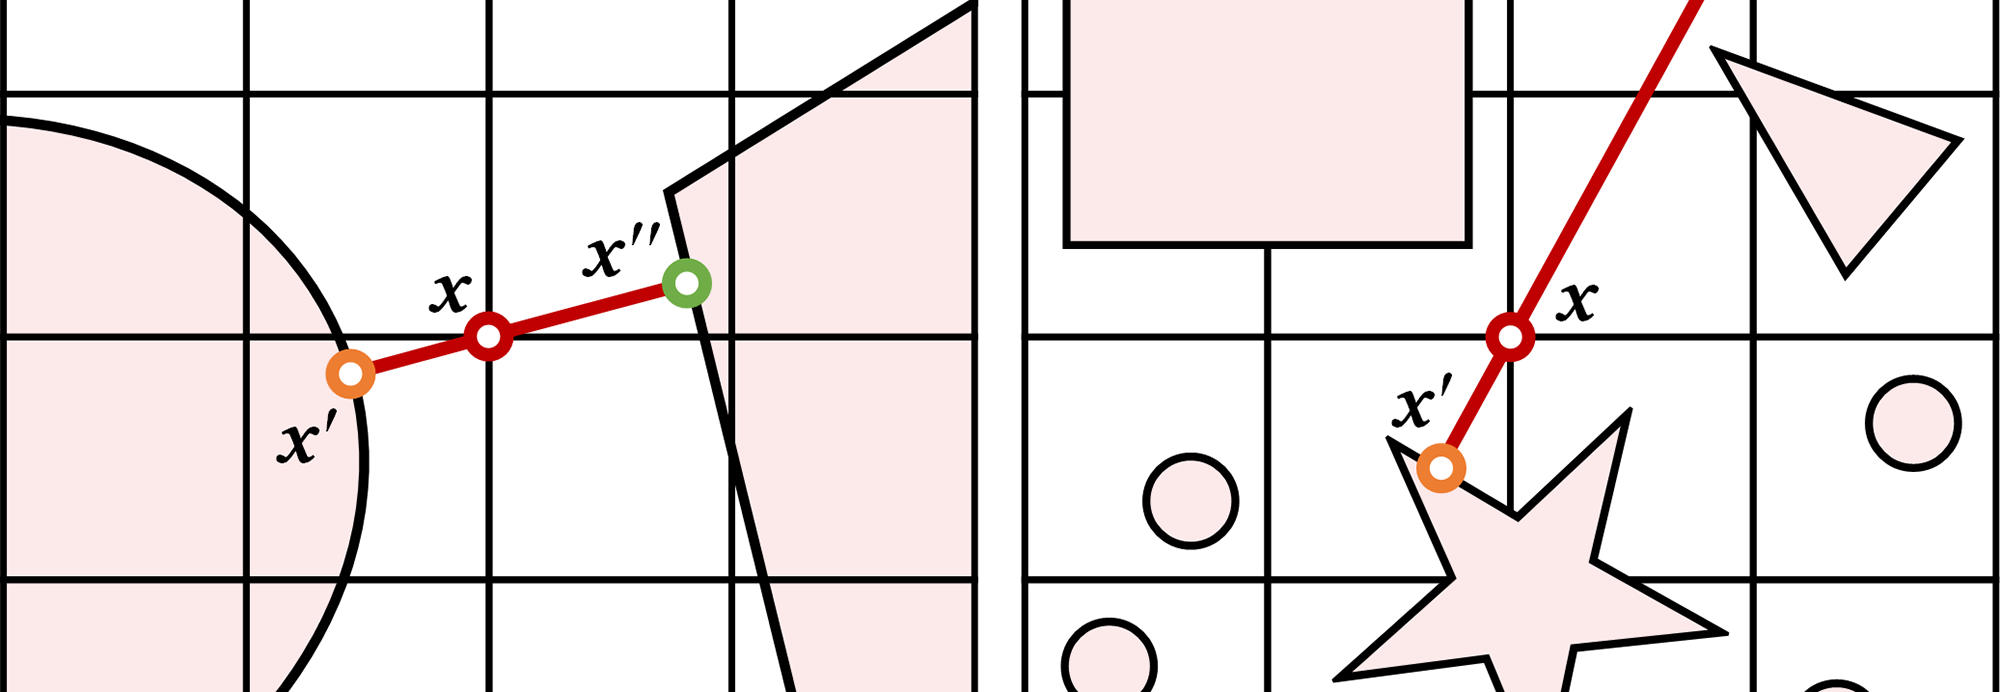
\includegraphics[width=0.95\columnwidth]{figures/cutcell_special_cases.png}
    \bicaption{两种邻近物体的情况。左图:从固体边界点$\bm{x}'$起始的射线经过$\bm{x}$点,在交到网格面之前,便相交于另一个物体上。这种情况,$\bm{x}''$是另一个固体边界点。右图:一个切削网格点可能完全被切削网格面包围,所以找不到任何非切削网格面。}{Two cases of solid proximity. Left: the ray starting from a boundary point $\bm{x}'$ through a grid node $\bm{x}$ may hit another boundary surface point before it intersects with the non-cut-cell face; in this case, $\bm{x}''$ locates at another boundary point. Right: a cut-cell node may be surrounded by all cut-cell faces, so a ray may not hit any non-cut-cell face nearby.}
    \label{img:handling_proximity}
\end{figure}

\paragraph{一些特殊情况}
% When solids are close to each other in the fluid compared to the size of a grid cell,
% there are a few cases where the velocity at $\bm{x}''$ \emph{cannot} be interpolated from nearby non-cut-cell nodes.
% Indeed, the ray from $\bm{x}'$ may hit the boundary of the same or another solid first (Fig.~\ref{fig:handling_proximity}, left).
% In this case, $\bm{x}''$ is defined as the first intersection along the ray with a boundary, and the solid velocity at this point is used in lieu of the bilinearly/trilinearly interpolated value described above; the final linear interpolation stays unchanged.
% Another case happens when the nearby axis-aligned faces intersected by the ray are all parts of cut-cells because of the proximity of different solids in the region (Fig.~\ref{fig:handling_proximity}, right).
% In this case, it becomes impossible to find a nearby reliable velocity with which to perform a linear interpolation, so we just discard the penalty force correction, and use only the approximation offered by the double-sided bounce-back process.

% \begin{figure}[b]\vspace*{-3.5mm}
% 	\centering 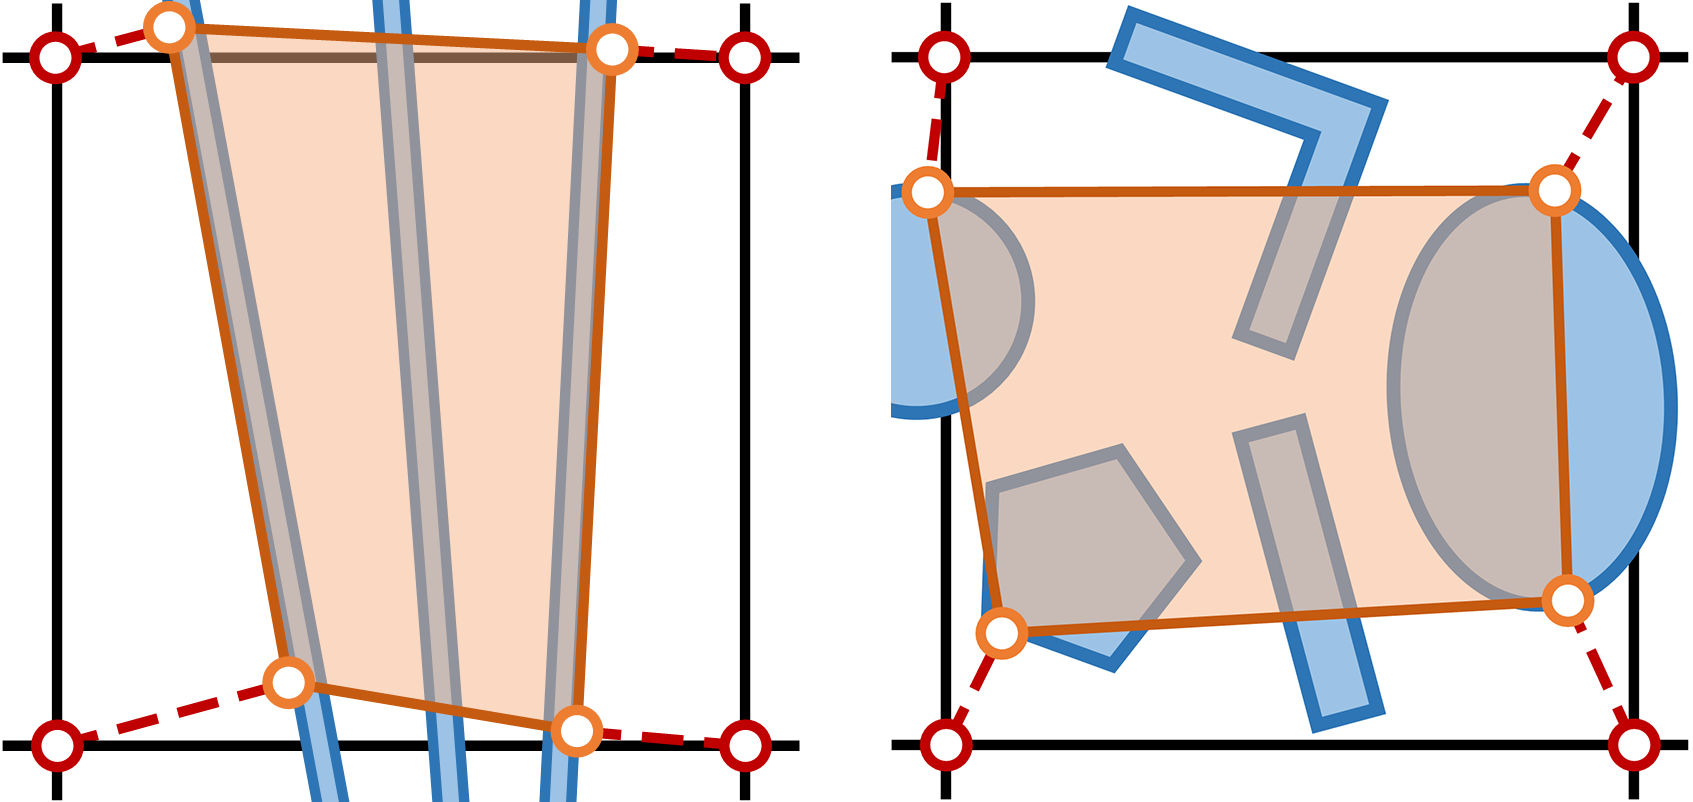
\includegraphics[width=0.9\columnwidth]{images/sub_grid_approximation} \vspace*{-2mm}
% 	\caption{\textbf{Sub-grid approximation.} To handle sub-grid scale solid structures, we project each cut-cell node onto its nearest boundary sample point. This basically amounts to using bounding volumes (orange regions) to approximate multiple thin structures within a cut-cell.
% 		\vspace*{-2mm}}
% 	\label{fig:sub_grid_approximation}
% \end{figure}

\paragraph{亚网格近似}
% Finally, in the case of thin shells or even thin rods being immersed in the fluid, it is possible that one fluid cell contains \emph{multiple} thin structures, especially when grid resolution is coarse relative to the spacing between structures (see Fig.~\ref{fig:sub_grid_approximation}) and cannot resolve the boundary condition accurately. As an efficient, yet reasonable approximation, we treat multiple thin structures inside a cut-cell as an immersed solid formed by the approximate bounding volumes they occupy. To this end, we just project each fluid cut-cell node to the nearest boundary point to compute the penalty force as described in Fig.~\ref{fig:sub_grid_approximation}. Note that this bounding volume approximation seamlessly handles stacked objects: while each object may have sub-grid thickness, the agglomerates act as a monolithic solid without the need for a specific treatment, see Fig.~\ref{fig:result-thin-shell-sub-grid}.

\paragraph{讨论}
% Our penalty force correction is based on linear velocity interpolation along the normal direction, effectively acting as a filter around solid boundaries to suppress spurious velocity oscillations generated by the bounce-back scheme at high Reynolds numbers.
% This correction significantly enhances the stability of two-way coupling in turbulent flow simulations, leading to visually plausible results even for relatively coarse grids. However, since it is only a first-order linear correction, high accuracy is only retained for sufficiently fine grid resolutions. Given that we target graphical applications, we do not consider more advanced models for velocity correction near solid boundaries in this work.

\subsection{固体受力}
% \label{sec:solid_force}
% Finally, we need to compute the momentum transfer from the surrounding fluid onto solids, which will be used to modify their motions for two-way coupling. Since we use a combination of bounce-back and velocity correction to derive the effects of the solids on the fluid, we must derive a new way to gather all the local fluid forces acting onto each solid in order to evaluate the resulting total force and torque exerted upon this solid.
% After our double-sided bounce-back treatment, we first accumulate all the momentum-exchange components from Eq.~\ref{eq:bounce-back} used during the double-sided bounce-back treatment for each cut-cell node inside fluid, then deduce the resulting total force and torque on each solid.
% More precisely, the momentum of fluid after streaming at node $\bm{x}$ and discrete time $t$ is expressed as: $\bm{p}(\bm{x}) = \sum_{i}\bm{c}_if^*_i(\bm{x},t)$.
% If $L$ is the set of all the ``cut-links'' (i.e., links intersecting the solid boundary at $\bm{x}$), for each cut-link $\bm{l}_j\in L$ where the bounce-back treatment has been applied, the momentum transferred to a solid in direction $\bm{c}_j$ is $\smash{-\bm{c}_{j}\,(f^*_{j}(\bm{x}) + f^*_{j'}(\bm{x}))}$. Therefore, the exchanged momentum $\Delta \bm{p}$ around $\bm{x}$ is: \vspace*{-1mm}
% \begin{equation}
% \Delta \bm{p}(\bm{x})= - \sum_{j\in L} \bm{c}_{j}\,(f^*_{j}(\bm{x}) + f^*_{j'}(\bm{x})), \vspace*{-1.5mm}
% \end{equation}
% where we did not explicitly write the multiplicative factor $(\Delta x)^3$ (where $\Delta x$ is the grid spacing) in front of the sum for simplicity, since it is always assumed to be 1 in normalized LBE space.
% The force acting on a solid by our double-sided bounce-back treatment can thus be approximated as the sum of all the momenta exchanged by all cut links that the solid intersects, leading to the expression: \vspace*{-1mm}
% \begin{equation}
% \bm{F}_{B}\equiv \sum_{\bm{x}} \Delta \bm{p}(\bm{x}), \vspace*{-1.25mm}
% \end{equation}
% where we removed a division by $\Delta t$ (the time step), which is also 1 in normalized LBE space. Similarly, the total torque is derived via:\vspace*{-1mm}
% \begin{equation}
% \bm{\tau}_{B}\equiv \sum_{\bm{x}} (\bm{x}-\bm{x}_{C})\times\Delta \bm{p}(\bm{x}). \vspace*{-1.25mm}
% \end{equation}
% where $\bm{x}_{C}$ is the center of mass of the solid object. \smallskip

% Note that the above forces and torques on solids we discussed thus far only account for our bounce-back treatment, thus only a portion of the entire coupling: our ancillary velocity correction (which also causes momentum change in cut-cells) exerts additional forces and torques on solids (albeit smaller) that should also be taken into account.
% We thus apply, at each time step, the opposite (reaction) penalty forces $\bm{F}_p$ from Eq.~\ref{eq:penaltyForce} onto the solids as typically done in DI-IB, resulting in a total correction force $\bm{F}_{C}$ and a total correction torque $\bm{\tau}_{C}$ induced by our velocity correction as: \vspace*{-1mm}
% \begin{equation}
% \bm{F}_{C} = - \sum_{\bm{x}}\bm{F}_p(\bm{x}), \quad \bm{\tau}_{C} = - \sum_{\bm{x}} (\bm{x}-\bm{x}_{C})\times\bm{F}_p(\bm{x}). \vspace*{-1mm}
% \end{equation}
% Finally, the total force $\bm{F}_s$ and torque $\bm{\tau}_s$ acting on a solid are the sum of the forces and torques we just described: \vspace*{-1mm}
% \[ \bm{F}_s = \bm{F}_{B} + \bm{F}_{C} \text{ and } \bm{\tau}_s = \bm{\tau}_{B} + \bm{\tau}_{C}. \]

\section{算法优化}
\subsection{几何近似}
% Our hybrid coupling method requires geometric computations, e.g., point projection onto, and intersections of links with, possibly complex solid surfaces, as well as the identification of cut-cells and their node classifications so that our velocity corrections can be applied. Many existing methods could be used to offer precise or even exact geometric calculations~\cite{Azevedo-2016,Robinson:2009}; however, they often significantly impact parallelism, drastically reducing the efficiency of the resulting LBM simulation.
% In order to compromise between accuracy and efficiency, we propose a sample-based approximation method which is of lower-order accuracy, but maintains the high degree of parallelism of traditional LBM. Moreover, visual simulation often does not necessitate very high accuracy (we will show however that our approach is still better at handling coupling in turbulent flows than most current CG techniques); but more accurate results can be obtained at the price of more computational time by increasing grid resolution.

% \begin{figure}[t]
% 	\centering 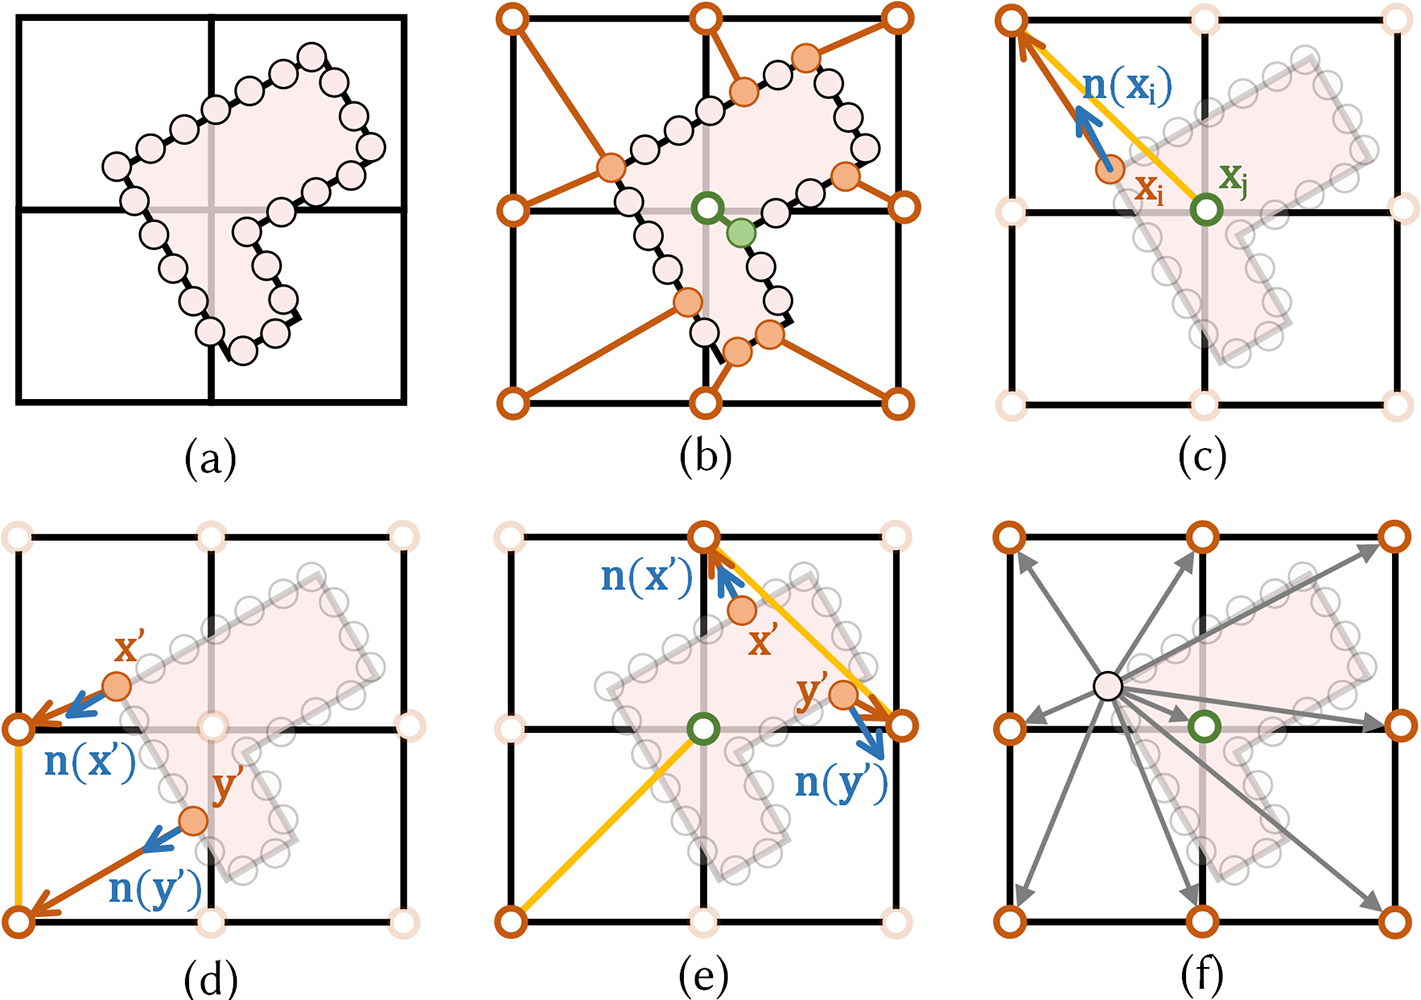
\includegraphics[width=0.95\columnwidth]{images/geometric_computing} \vspace*{-3.5mm}
% 	\caption{\textbf{Efficient geometric approximation}. Given a solid geometry, we first sample its boundary (a); then the projected points of cut-cell nodes can be simply approximated by the nearest sample (b). To examine whether a link (yellow) crosses the solid boundary, we first check if solid nodes are involved. If the ends of the link are fluid and solid nodes, then it crosses the solid boundary (c) (green cut-cell nodes are inside the solid, whereas orange ones are in the fluid). For links connecting fluid nodes, we check the normals of the two projected cut-cell nodes forming the link; if the two normals have the same orientation (d), the link does not cross the solid boundary; otherwise, it intersects the solid boundary (e). For GPU implementation, we parallelize over solid samples instead of cut-cell nodes, where each solid sample will check its surrounding region of cut-cell nodes.
% 	\vspace*{-3mm}}
% 	\label{fig:geometric-computing}
% \end{figure}

% \paragraph{Surface sampling and cut-cell identification}
% Instead of using the real geometry of boundaries, we first uniformly \emph{sample} all solid boundary surface meshes --- for instance via Poisson-disk sampling~\cite{dunbar2006spatial}; note that the surface mesh should be watertight to facilitate this sample-based treatment. Each sample point $\bm{x}_s$ is then equipped with a \emph{normal} $\bm{n}(\bm{x}_s)$, set to be the outward boundary normal at this point. We then declare a cell to be a \emph{cut-cell} if it contains \emph{at least one boundary sample}, which is simple and fast to evaluate, see Fig.~\ref{fig:geometric-computing} (a) for a 2D example.

% \begin{figure*}[t]
% 	\centering 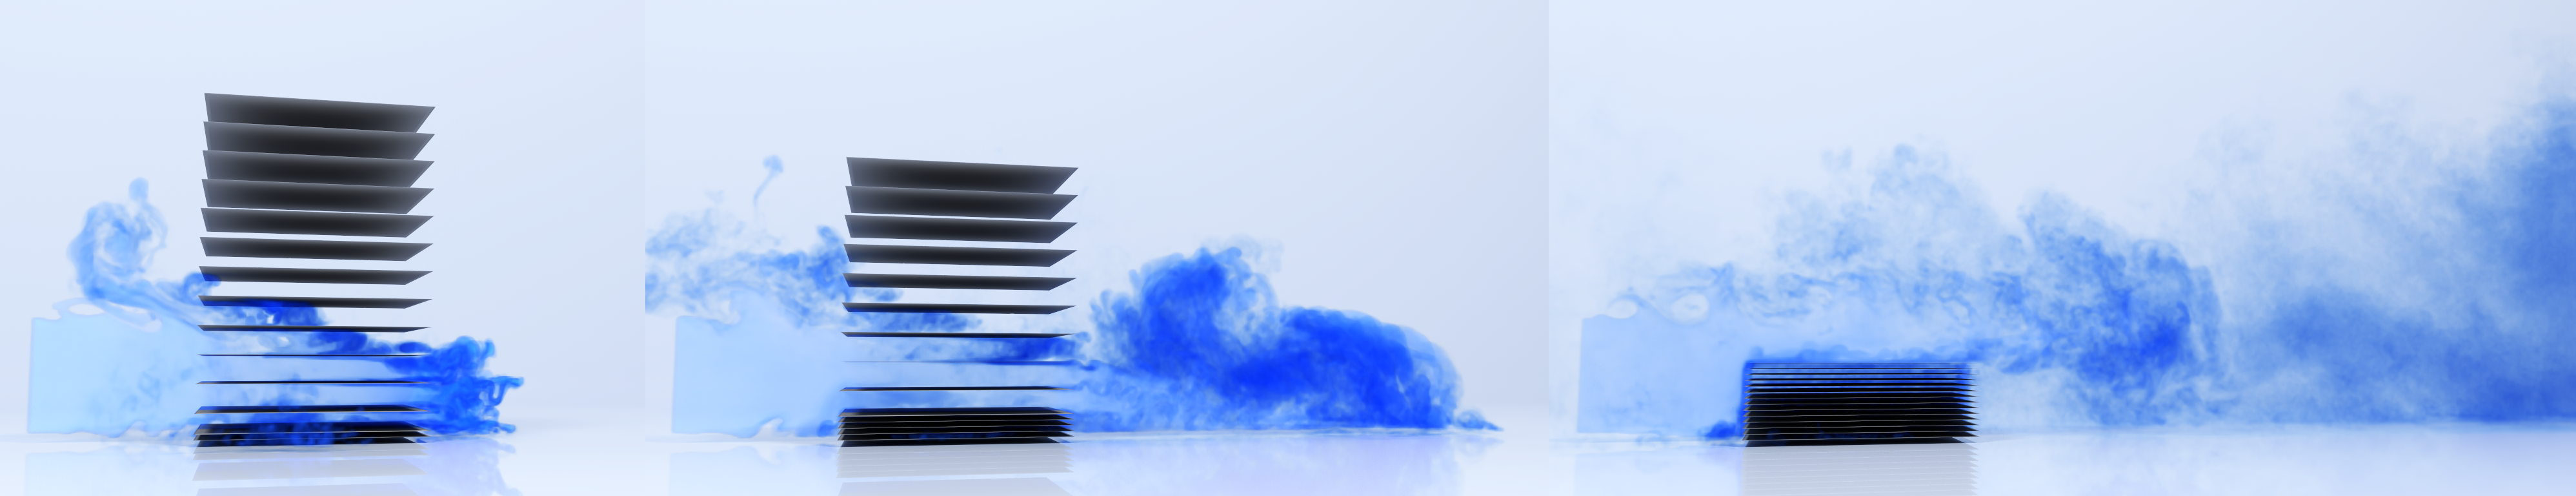
\includegraphics[width=0.99\textwidth]{images/result_thin_shell_sub_grid} \vspace*{-3mm}
% 	\caption{\textbf{Smoke flow through stacked plates}. Smoke is blown towards a falling stack of thin plates. While smoke freely flows between separate plates, they become an airtight obstacle when they are stacked on top of each other. Our boundary treatment based on subgrid approximation deals with both cases seamlessly: plates getting closer accelerate the flow in between them, while tightly stacked plates are treated as thick solids.
% 		\vspace*{-2.5mm}}
% 	\label{fig:result-thin-shell-sub-grid}
% \end{figure*}

% \paragraph{Efficient cut-cell node projection}
% One of the most important (and potentially time-consuming) geometric computations is to project nodes $\bm{x}$ that lie in the fluid and belong to a cut-cell onto the solid boundary surface in order to compute their projection $\bm{x}'$, which will be used in both our double-sided bounce-back scheme and ancillary velocity correction. For boundaries described through a surface mesh, this is traditionally achieved by constructing a tree structure from the boundary mesh and searching the nearest triangle~\cite{wang-2012}; instead, our sampling of the boundary allows us to replace this projection procedure by an approximate, but very efficient algorithm: for each fluid node of a cut-cell,  we pick the nearest sample $\bm{x}_s$ satisfying\vspace*{-1mm}
% \begin{equation}\label{eq:is_in_fluid}
% (\bm{x}-\bm{x}_s)\cdot \bm{n}(\bm{x}_s) \geq 0\; \vspace*{-0.5mm}
% \end{equation}
% to approximate the projected point $\bm{x}'$ --- this constraint preventing the selection of samples that do not \emph{face} the node.
% If no samples can be found, then the node is marked as a solid node;
% see the green node of Fig.~\ref{fig:geometric-computing} (b) for a 2D case.
% This sample-based technique is efficient and easily parallelizable, but the accuracy obviously depends on sample density;
% in practice, we ensure sufficient samples per cut-cell such that the approximation is still accurate by picking an appropriate minimum distance for the Poisson-disk sampling, typically set to half a grid cell size.

% \paragraph{Approximate bounce-back scheme}
% In our double-sided bounce-back scheme, one must identify links that intersect a solid boundary (Fig.~\ref{fig:bounce_back_scheme}).
% For thick solids, since we have already identified whether cut-cell nodes are inside the solid, we only need to check the two end nodes of a link: if one of these two nodes is a fluid node and the other is a solid node, the link clearly intersects a solid boundary, and the DSBB scheme must be applied for that link instead of the regular streaming.
% However, for thin shells, all the nodes on a cut-cell are fluid nodes. Therefore, we proceed as follows.
% Given a link between node $\bm{x}$ and $\bm{y}$, we check \emph{whether the normals of the two projected points $\bm{x}'$ and $\bm{y}'$ point in opposite directions}, i.e., $\bm{n}(\bm{x}')\!\cdot\!\bm{n}(\bm{y'})\!<\!0$, see Fig.~\ref{fig:geometric-computing} (d) and (e).
% If this last condition holds (Fig.~\ref{fig:geometric-computing} (e) shows two situations for a link crossing a solid boundary), $\bm{x}$ and $\bm{y}$ are on two different sides of a shell and the link is tagged as intersecting a boundary, and the DSBB scheme is then applied.

\subsection{GPU实现}
% All of our algorithms so far, including geometric approximations, are designed to involve \emph{purely local computations} with relatively simple algebra. It results in an overall coupling approach that is straightforward to implement on a parallel computing platform such as a GPU for efficient simulation: it respects the embarrassingly parallel nature of LBM. Our simulation method is very scalable since it can run on either a single or multiple GPU(s) by leveraging the GPU optimization techniques presented in \cite{Chen-2021}; our examples are computed with only one GPU, except for a high-resolution simulation shown in Fig.~\ref{fig:result-city} where we used two GPUs instead. We discuss next a few specific accelerations and optimizations we incorporated in our GPU implementation in order to improve the overall performance for our two-way coupled simulations. \vspace*{-1mm}

% \paragraph{Memory layout}
% For LBM, a structure-of-arrays (SoA) memory layout is recommended to store discrete distribution functions $f_i$ of all grid nodes to improve cache utilization and thus improve performance~\cite{Chen-2021}. We follow this recommendation in our GPU implementation as our tests showed that the SoA layout is still the most efficient, even with our new coupling strategy. \vspace*{-1.5mm}

% \paragraph{Efficient collision evaluation}
% Also discussed and demonstrated in~\cite{Chen-2021} was the computation of the inverse of the central-moment projection matrix $\bm{M}(\bm{u})$. They argued that this inverse should be computed analytically to preserve accuracy, but the algebraic expression is very lengthy and occupies many registers, resulting in low achieved GPU occupancy in practice.
% However, we observed that if one performs an analytical LU decomposition~\cite{fei2018three} of $\bm{M}(\bm{u})^{-1}$, many elements of the resulting triangular matrices are very close to zero. Thus, we can discard those close-to-zero elements and employ the usual sparse matrix format to store the decomposed matrices, decreasing drastically the terms needed to compute the inverse. This does not influence accuracy (the reconstruction error is below machine accuracy), but significantly reduces the use of registers; the performance for parallel collision calculation is then three times faster on average compared to the implementation using~\cite{Chen-2021} on the same GPU. \vspace*{-1.5mm}

% \paragraph{Parallel cut-cell point projection and identification}
% Throughout all the stages of our hybrid coupling algorithm, a key operation is to project a cut-cell node onto the nearest solid boundary, which is approximated by searching for the nearest sample point on the solid boundaries.
% While there are traditional
% GPU implementations to achieve this task in parallel over cut-cell nodes, they often generate load imbalance and low GPU occupancy issues.
% %as pointed out in~\cite{Chen-2021} for their case of a GPU-based immersed boundary method.
% Thus, as suggested in \cite{Chen-2021}, we parallelize over solid samples instead --- but proceed differently to improve performance.
% For each sample, we compute the distance to each node of the cut cell in which the sample is located (see Fig.~\ref{fig:geometric-computing} (f)) and compare with the distance stored in that node: if the distance of the sample to a cut-cell node is smaller than the current distance stored in that node, we update this distance with the new distance, and change the index of the solid sample stored along with that same node.
% Since the same cut-cell node may be accessed from multiple solid sample threads, we employ an atomic comparison operation to avoid thread conflicts.
% Note that Eq.~\eqref{eq:is_in_fluid} still needs to be satisfied for every comparison, so the identification of solid nodes is included in the process.
